\documentclass[aspectratio=169,11pt]{beamer}

\usetheme{default}
\usecolortheme{default}
\usepackage{tikz}
\usetikzlibrary{calc}
% Comandos compartidos entre slides.tex y handout.tex
\usepackage{amsmath,amssymb}
\usepackage{siunitx}
\usepackage{booktabs}
\sisetup{per-mode=symbol}

\newcommand{\kB}{k_B}
\newcommand{\DG}{\Delta G}
\newcommand{\DGd}{\Delta G^{\ddagger}}
\newcommand{\Feq}{F_{\text{eq}}}
\newcommand{\peq}{p_{\text{eq}}}
\newcommand{\bhat}{\hat{F}}

% paleta sobria compartida (mismos tonos que el diagrama TikZ)
\definecolor{miazul}{RGB}{31,79,121}
\definecolor{minaranja}{RGB}{204,102,0}
\definecolor{migris}{RGB}{90,90,90}

% pie de figura compacto -- reutilizado en slides.tex y handout.tex
\newcommand{\Pie}[1]{%
  \vspace{0.4em}
  \begin{center}
  \begin{minipage}{0.82\textwidth}
    \centering{\scriptsize\color{migris}\itshape #1}
  \end{minipage}
  \end{center}%
}

\graphicspath{{../assets/}{figs/}}
% Diagrama de 3 paneles: paisaje real -> sesgo acumulado -> efecto neto plano
% Idea: el sesgo bien-templado converge a un "molde negativo" de F(s).
% Uso: \MoldeNegativoFigure[<scale>]
\newcommand{\MoldeNegativoFigure}[1][1]{%
\begin{tikzpicture}[scale=#1, every node/.style={font=\small}]

  % ---------- Panel 1: F(s) ----------
  \begin{scope}[xshift=0cm]
    \draw[->] (-0.3,0) -- (5.3,0) node[right] {\scriptsize $s$};
    \draw[->] (0,-0.3) -- (0,3.3) node[above] {\scriptsize $F(s)$};
    \draw[thick, blue!55!black, smooth, tension=0.85] plot coordinates {
      (0,2.6) (0.6,1.6) (1.1,0.35) (1.7,1.3) (2.3,2.9) (3.0,1.3) (3.6,0.85) (4.2,1.7) (4.8,2.7)
    };
    \node at (1.1,-0.6) {\scriptsize $A$};
    \node at (3.6,-0.6) {\scriptsize $B$};
    \node at (2.3,3.15) {\scriptsize barrera};
    \node[align=center] at (2.4,-1.15) {\footnotesize\bfseries Paisaje real};
  \end{scope}

  \draw[->, thick] (5.55,1.5) -- (6.35,1.5);

  % ---------- Panel 2: V(s,t) creciendo con el tiempo ----------
  \begin{scope}[xshift=6.7cm]
    \draw[->] (-0.3,0) -- (5.3,0) node[right] {\scriptsize $s$};
    \draw[->] (0,-0.3) -- (0,3.3) node[above] {\scriptsize $V(s,t)$};
    % fondo tenue: forma de -F(s), de referencia
    \draw[gray!35, smooth, tension=0.85] plot coordinates {
      (0,0.4) (0.6,1.4) (1.1,2.65) (1.7,1.7) (2.3,0.1) (3.0,1.7) (3.6,2.15) (4.2,1.3) (4.8,0.3)
    };
    % t1 (mas tenue, mas bajo)
    \draw[orange!40, smooth, tension=0.85] plot coordinates {
      (0.65,0) (1.1,0.85) (1.55,0) (3.25,0) (3.6,0.5) (3.95,0)
    };
    % t2 (medio)
    \draw[orange!70, smooth, tension=0.85] plot coordinates {
      (0.55,0) (1.1,1.65) (1.65,0) (3.15,0) (3.6,1.0) (4.05,0)
    };
    % t3 (mas oscuro, mas alto -- ya casi rellena los pozos de F(s))
    \draw[orange!95!black, thick, smooth, tension=0.85] plot coordinates {
      (0.45,0) (1.1,2.45) (1.75,0) (3.05,0) (3.6,1.55) (4.15,0)
    };
    \node[anchor=south west, align=left, font=\scriptsize] at (0.1,2.85) {$t_1 < t_2 < t_3$};
    \node[align=center] at (2.4,-1.15) {\footnotesize\bfseries Sesgo acumulado};
  \end{scope}

  \draw[->, thick] (12.35,1.5) -- (13.15,1.5);
  \node[align=center, font=\scriptsize] at (12.75,1.85) {$F+V$};

  % ---------- Panel 3: F(s)+V(s) practicamente plano ----------
  \begin{scope}[xshift=13.5cm]
    \draw[->] (-0.3,0) -- (5.3,0) node[right] {\scriptsize $s$};
    \draw[->] (0,-0.3) -- (0,3.3) node[above] {};
    \draw[blue!55!black, thick, smooth, tension=0.85] plot coordinates {
      (0,1.55) (0.8,1.48) (1.6,1.62) (2.4,1.5) (3.2,1.6) (4.0,1.48) (4.8,1.55)
    };
    \node[align=center] at (2.4,-1.15) {\footnotesize\bfseries Efecto neto};
    \node[align=center, font=\scriptsize] at (2.4,0.55) {el sistema difunde libremente};
  \end{scope}

\end{tikzpicture}%
}


% ---------- tema sobrio ----------
\setbeamertemplate{navigation symbols}{}
\setbeamertemplate{headline}{}
\setbeamertemplate{footline}{%
  \hspace{1em}\usebeamercolor[fg]{structure}{\tiny Inventando la metadinámica}%
  \hfill%
  \tiny\insertframenumber{}/\inserttotalframenumber\hspace{1.2em}\vskip 3pt
}
\setbeamercolor{frametitle}{fg=miazul}
\setbeamercolor{title}{fg=miazul}
\setbeamercolor{structure}{fg=miazul}
\setbeamercolor{alerted text}{fg=minaranja}
\setbeamertemplate{itemize items}{\textcolor{minaranja}{\footnotesize\textbullet}}
\setbeamertemplate{itemize subitem}{\textcolor{migris}{\scriptsize\textbullet}}
\setbeamerfont{frametitle}{series=\bfseries,size=\large}
\setbeamerfont{title}{series=\bfseries}
\setbeamertemplate{blocks}[rounded][shadow=false]
\setbeamercolor{block title}{fg=white,bg=miazul}
\setbeamercolor{block body}{fg=black,bg=miazul!6}

\newcommand{\Fuente}[1]{{\scriptsize\color{migris} #1}}

\title{Inventando la metadinámica}
\subtitle{Metodología de Fernández-Quintero \emph{et al.} (2022) — humanización de VNARs de tiburón}
\author{}
\date{\today}

\begin{document}

% ===================================================================
\begin{frame}
  \titlepage
  \vspace{-1em}
  \begin{center}
    \small Fernández-Quintero ML, Fischer A-LM, Kokot J, Waibl F, Seidler CA, Liedl KR.\\
    \textit{The influence of antibody humanization on shark variable domain (VNAR) binding site ensembles.}\\
    Front. Immunol. \textbf{13}:953917 (2022)
  \end{center}
\end{frame}

% ===================================================================
\section{El sistema}

\begin{frame}{El dominio de unión más pequeño que existe}
  \begin{columns}[T]
    \begin{column}{0.55\textwidth}
      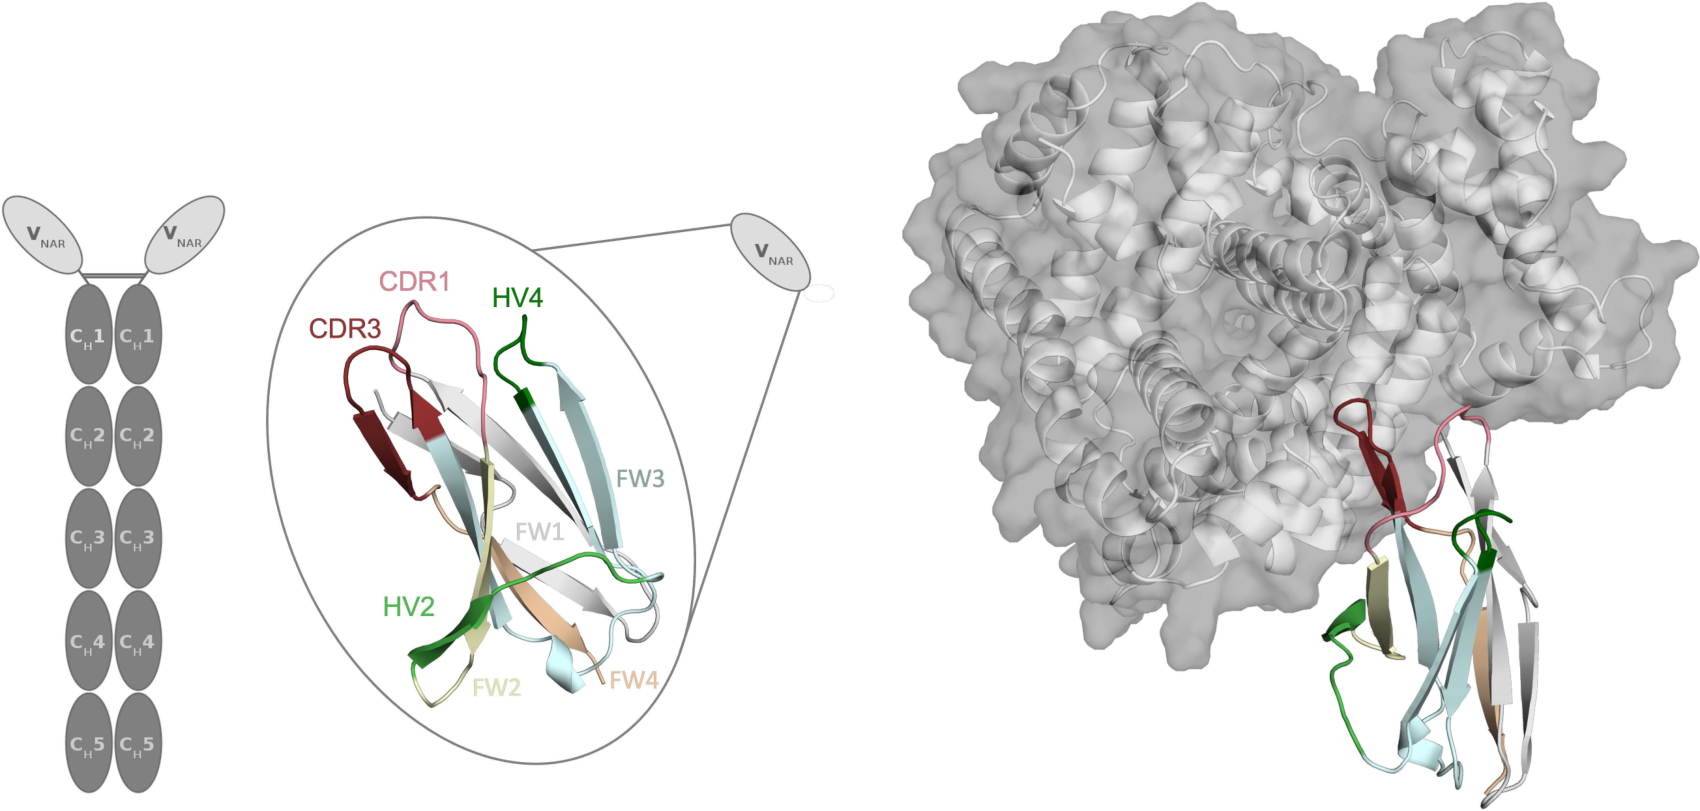
\includegraphics[width=\textwidth]{fig1-vnar-estructura.png}
    \end{column}
    \begin{column}{0.45\textwidth}
      \begin{itemize}
        \item \textbf{IgNAR}: anticuerpo de tiburón, homodímero, \alert{solo cadena pesada}
        \item El dominio variable aislado: \textbf{VNAR}
        \item Un Fv convencional tiene \textbf{6} CDRs (VH+VL). Un VHH (nanobody), \textbf{3}.
        \item Un VNAR: \alert{solo 2} — CDR1 y CDR3
        \item La CDR2 falta (sin hebras C$'$/C$''$) — compensada por \textbf{HV2} y \textbf{HV4}
      \end{itemize}
    \end{column}
  \end{columns}
\end{frame}

\begin{frame}{Humanizar: tocar el framework, no las CDRs}
  \begin{columns}[T]
    \begin{column}{0.55\textwidth}
      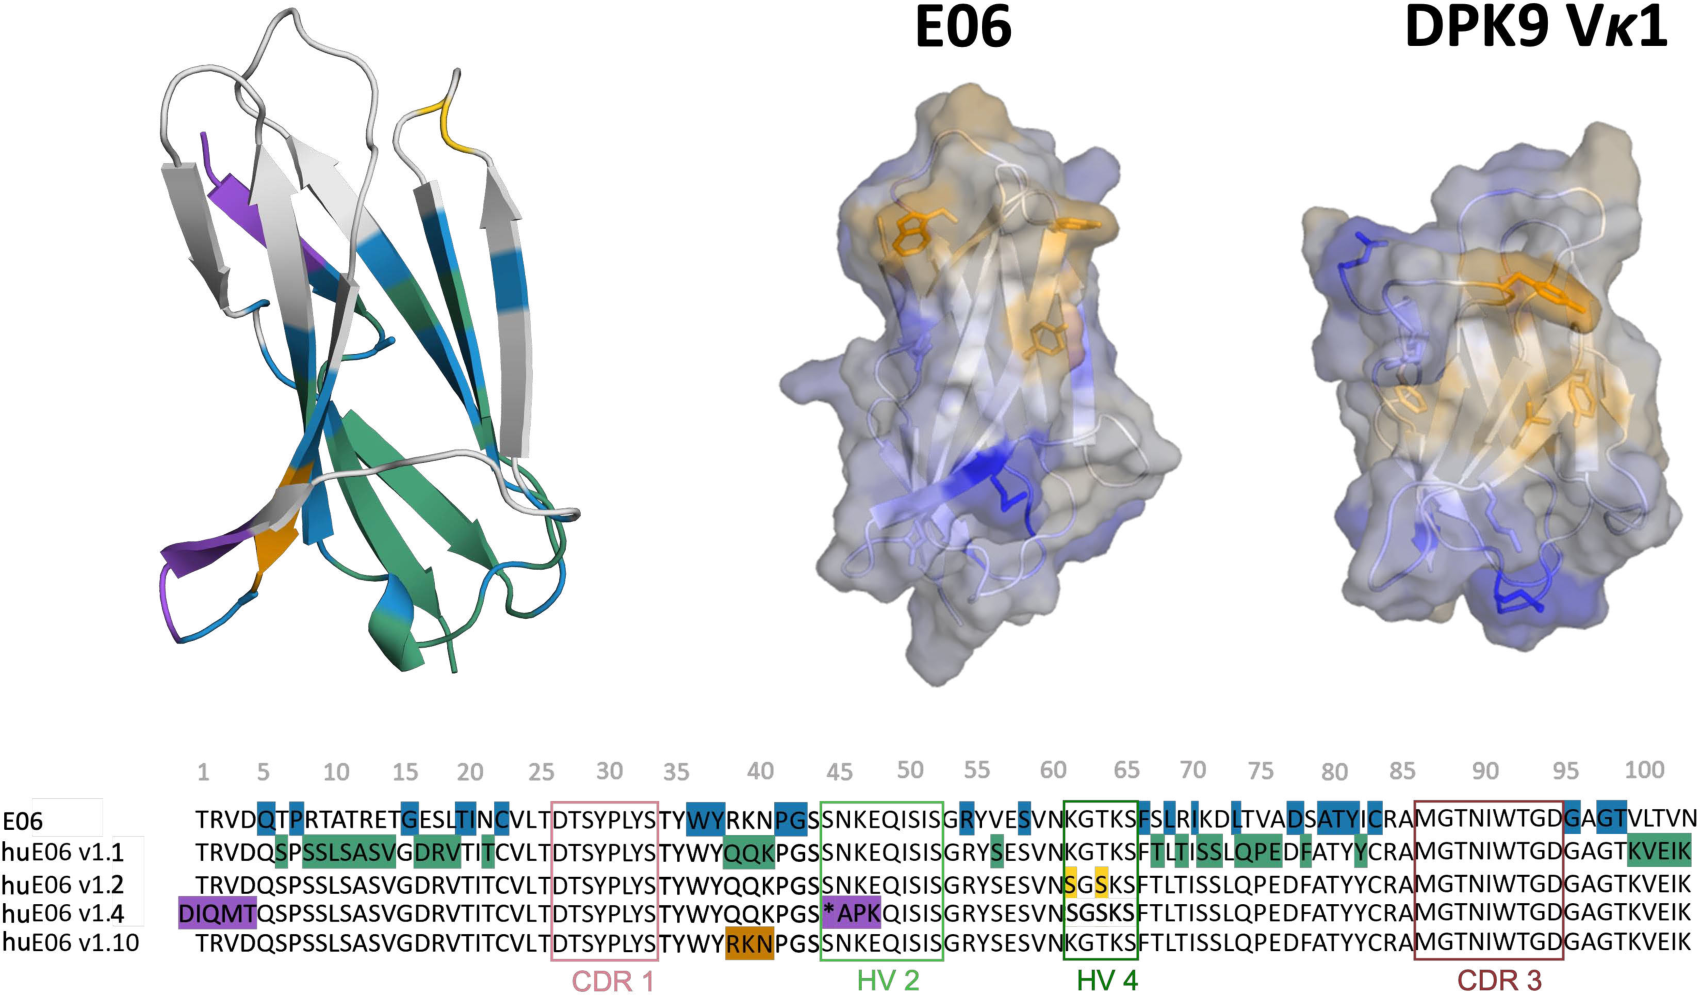
\includegraphics[width=\textwidth]{fig2-alineamiento-hidrofobicidad.png}
    \end{column}
    \begin{column}{0.45\textwidth}
      \begin{itemize}
        \item \textbf{E06} (mielga) $\to$ variantes humanizadas v1.1 $\to$ v1.2 $\to$ v1.4
        \item Referencia humana: \textbf{DPK9}, germinal V$\kappa$1
        \item \textbf{v1.10} revierte el motivo \texttt{RKN} — control interno de reversión
        \item DPK9 es cadena \emph{ligera}: en un Fab tiene cara hidrofóbica de apareamiento con VH
        \item El VNAR vive \textbf{solo} — esa cara queda expuesta
      \end{itemize}
    \end{column}
  \end{columns}
\end{frame}

\begin{frame}{La pregunta}
  \begin{center}
    \Large
    Humanizar cambia la afinidad.\\[0.6em]
    \alert{¿Cambia también el \emph{ensemble} conformacional?}\\[1.2em]
    \normalsize
    \color{migris}
    ¿Cómo se comprueba eso computacionalmente?
  \end{center}
\end{frame}

% ===================================================================
\section{El problema}

\begin{frame}{Poblaciones = pesos de Boltzmann}
  \begin{block}{La única definición que necesitamos}
    $$\frac{P_A}{P_B} = e^{-\Delta G_{AB}/RT} \qquad\Longleftrightarrow\qquad \Delta G_{AB} = -RT\ln\frac{P_A}{P_B}$$
  \end{block}
  \vspace{0.5em}
  \begin{itemize}
    \item A 300 K: $RT \approx \SI{2.5}{\kilo\joule\per\mole}$
    \item Regla práctica: \alert{un factor $e$ en población cuesta 2.5 kJ/mol}
    \item Un factor 10 cuesta $RT\ln 10 \approx \SI{5.7}{\kilo\joule\per\mole}$
  \end{itemize}
  \vspace{0.5em}
  \Fuente{Sin matices: es la definición del ensemble canónico.}
\end{frame}

\begin{frame}{¿Por qué la MD directa no basta?}
  \begin{block}{Teoría del estado de transición}
    $$k = \kappa\,\frac{k_BT}{h}\,e^{-\Delta G^{\ddagger}/RT}, \qquad \tau = 1/k$$
  \end{block}
  \begin{center}
  \begin{tabular}{ccc}
    \toprule
    $\Delta G^{\ddagger}$ & $\tau$ (estimado) & ¿cruza en 100 ns? \\
    \midrule
    20 kJ/mol & $\sim$30 ns & sí, varias veces \\
    \alert{$\sim$22 kJ/mol} & \alert{$\sim$100 ns} & \alert{frontera} \\
    40 kJ/mol & $\sim$90–150 $\mu$s & \textbf{no} \\
    \bottomrule
  \end{tabular}
  \end{center}
  \vspace{0.8em}
  \textbf{100 ns de MD compran barreras de hasta $\sim$22 kJ/mol.} Las transiciones de lazos CDR viven en 25–45 kJ/mol.
\end{frame}

\begin{frame}{El resultado que hay que poder explicar}
  \centering
  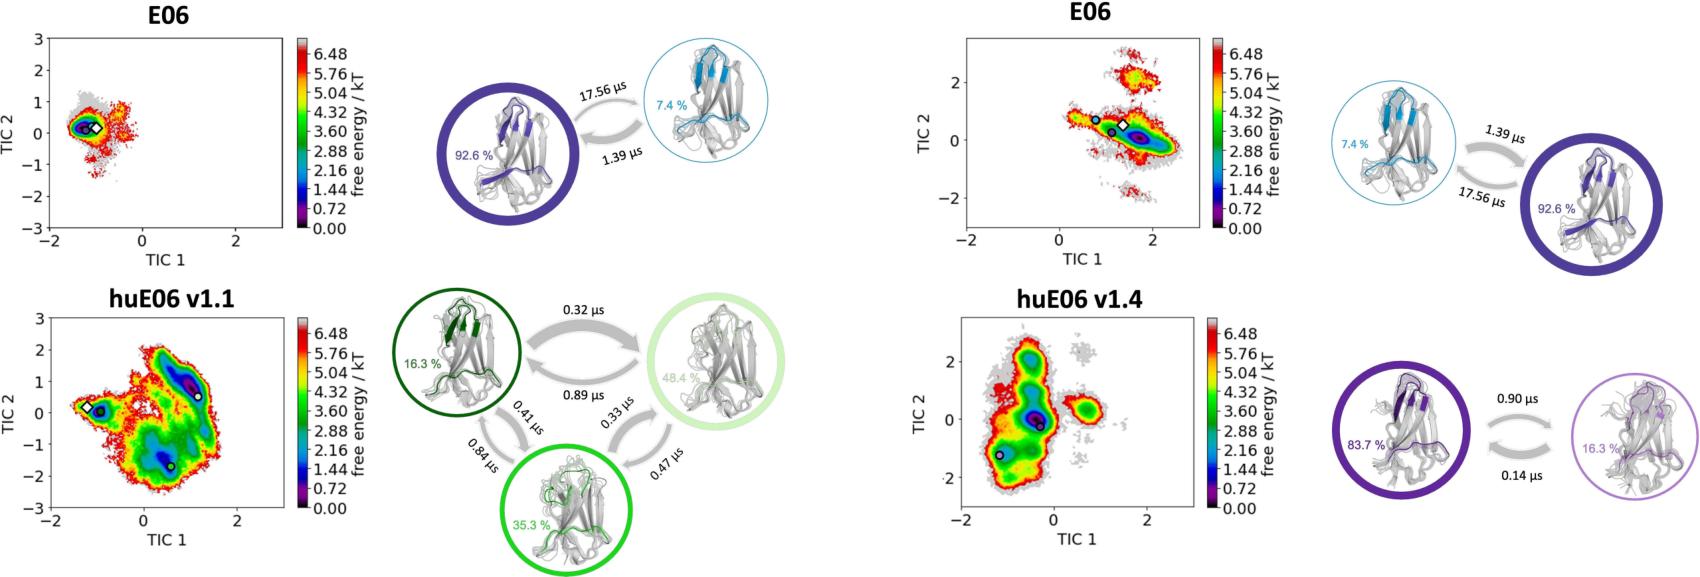
\includegraphics[width=0.92\textwidth]{fig4-msm-poblaciones.png}\\[0.3em]
  {\scriptsize E06: \textbf{92.6\%} / 7.4\% \quad$\to$\quad huE06 v1.1: 16.3\% / 48.4\% / 35.3\%}
  \vspace{0.4em}

  \alert{$\Delta\Delta G \approx 10$ kJ/mol} — comparable al error típico de un campo de fuerza en energías conformacionales de lazos
\end{frame}

\begin{frame}{Conclusión del Bloque 1}
  \begin{center}
    \Large
    Necesitamos cruzar barreras de $\sim$40 kJ/mol\\
    sin esperar $\sim$100 $\mu$s por cruce\\[0.6em]
    \alert{sin destruir las poblaciones al hacerlo.}
  \end{center}
\end{frame}

% ===================================================================
\section{Inventar la metadinámica}

\begin{frame}{¿Qué palancas existen?}
  \begin{columns}[T]
    \begin{column}{0.48\textwidth}
      \textbf{Temperatura global (REMD)}
      \begin{itemize}
        \item[\textcolor{minaranja}{$-$}] acelera \emph{todo} indiscriminadamente
        \item[\textcolor{minaranja}{$-$}] reponderar a 300 K es caro (varianza $\sim e^{\sqrt{N}}$)
        \item[\textcolor{minaranja}{$-$}] no se puede apuntar a un lazo
        \item[\textcolor{teal}{$+$}] no requiere elegir CVs
      \end{itemize}
    \end{column}
    \begin{column}{0.48\textwidth}
      \textbf{Sesgar el potencial sobre una CV}
      \begin{itemize}
        \item[\textcolor{teal}{$+$}] selectivo — solo empuja donde uno decide
        \item[\textcolor{teal}{$+$}] el sesgo se conoce exactamente: barato de quitar
        \item[\textcolor{minaranja}{$-$}] hay que \alert{elegir} las CVs de antemano
      \end{itemize}
    \end{column}
  \end{columns}
  \vspace{1em}
  \centering \alert{\large Metadinámica: sesgar sobre la CV.}
\end{frame}

\begin{frame}{Un sesgo sobre la CV se suma al paisaje}
  Si $U_V(\mathbf{r}) = U(\mathbf{r}) + V(\xi(\mathbf{r}))$, entonces \textbf{exactamente}:
  $$\boxed{F_V(s) = F(s) + V(s)}$$
  \vspace{0.4em}
  \begin{itemize}
    \item Se cumple porque $V$ depende de $\mathbf{r}$ \emph{solo a través de} $s=\xi(\mathbf{r})$
    \item El sesgo que aplana el paisaje: $F_V = 0 \iff V(s) = -F(s)$
  \end{itemize}
  \begin{alertblock}{El problema}
    Para construir $V=-F$ hace falta conocer $F$ — que es justo lo que queremos medir. \textbf{Huevo y gallina.}
  \end{alertblock}
\end{frame}

\begin{frame}{La solución: sesgo adaptativo}
  Depositar, cada $\tau_G$ pasos, una gaussiana donde está el sistema \emph{ahora}:
  $$V(s,t) = \sum_{t' < t} W\, e^{-(s-\xi(\mathbf{r}(t')))^2/2\sigma^2}$$
  \vspace{0.3em}
  \begin{itemize}
    \item El sistema \textbf{va dejando arena donde pisa}
    \item Bucle de realimentación: $\dfrac{\partial V}{\partial t} \propto e^{-\beta[F(s)+V(s,t)]}$
    \item Pozo profundo $\to$ más tiempo ahí $\to$ deposita rápido $\to$ se autolimita
  \end{itemize}
  \begin{alertblock}{Pero...}
    La deposición \textbf{nunca para}. El sistema acaba explorando regiones absurdas (\emph{overfilling}).
  \end{alertblock}
\end{frame}

\begin{frame}{El sesgo como molde negativo del paisaje}
  \centering
  \resizebox{\textwidth}{!}{\MoldeNegativoFigure[1]}
\end{frame}

\begin{frame}{Well-tempered: frenar la deposición}
  La altura decae donde ya hay sesgo: $W(s,t) = W_0\, e^{-V(s,t)/k_B\Delta T}$
  \vspace{0.3em}
  \begin{block}{Convergencia}
    $$V(s) \xrightarrow[t\to\infty]{} -\frac{\gamma-1}{\gamma}F(s), \qquad \gamma \equiv \frac{T+\Delta T}{T}$$
  \end{block}
  \begin{columns}[T]
    \begin{column}{0.5\textwidth}
      \begin{itemize}
        \item Barrera residual: $F_V = F/\gamma$
        \item Muestreo: $p_V \propto \peq^{\,1/\gamma}$
      \end{itemize}
    \end{column}
    \begin{column}{0.5\textwidth}
      \begin{itemize}
        \item Recuperar $F$: $F = -\dfrac{\gamma}{\gamma-1}V$
        \item $\gamma\to 1$: MD normal. $\gamma\to\infty$: metaD estándar
      \end{itemize}
    \end{column}
  \end{columns}
\end{frame}

\begin{frame}{Los números del paper}
  \begin{center}
  \begin{tabular}{ll}
    \toprule
    CVs & $\sin\psi,\cos\psi$ de CDR1 y CDR3 \\
    Biasfactor $\gamma$ & 10 \quad ($\Delta T = 2700$ K) \\
    Altura / ancho gaussiana & 10 kJ/mol / 0.3 rad \\
    Deposición & cada 2 ps \\
    Duración & 1 $\mu$s por sistema \\
    \bottomrule
  \end{tabular}
  \end{center}
  \vspace{0.8em}
  \centering
  Barrera 40 kJ/mol $\xrightarrow{\ \gamma=10\ }$ \alert{4 kJ/mol}
  \qquad
  Aceleración $\approx \mathbf{1.9\times10^{6}}$
\end{frame}

% ===================================================================
\section{El precio}

\begin{frame}{La cinética queda comprimida, no solo cambiada}
  Factor de aceleración por transición: $\alpha = e^{\beta\Delta G^{\ddagger}(\gamma-1)/\gamma}$ — \alert{depende de la barrera}
  $$\frac{\tau_A^V}{\tau_B^V} = \left(\frac{\tau_A}{\tau_B}\right)^{1/\gamma}$$
  \vspace{0.3em}
  \begin{exampleblock}{Ejemplo}
    Si en el sistema real $A$ tarda \textbf{23\,000$\times$} más que $B$, sesgado con $\gamma=10$:
    $$23\,000^{1/10} \approx \mathbf{2.7}$$
  \end{exampleblock}
  \textbf{Cuatro órdenes de magnitud, aplastados a un factor 3.} No es un efecto secundario — es el mecanismo.
\end{frame}

\begin{frame}{Las CVs son una elección}
  La fuerza de sesgo sobre el átomo $i$: $\mathbf{f}_i = -\dfrac{dV}{ds}\,\nabla_{\mathbf{r}_i}\xi(\mathbf{r})$
  \begin{itemize}
    \item Si el átomo $i$ no define la CV: $\nabla_{\mathbf{r}_i}\xi = \mathbf{0}$
    \item El sesgo empuja \textbf{literalmente} solo los átomos de CDR1/CDR3
    \item Todo grado de libertad ortogonal (p. ej. HV2) recibe \alert{ayuda cero}
  \end{itemize}
  \vspace{0.5em}
  \Fuente{No es una sutileza — es una restricción mecánica del método.}
\end{frame}

\begin{frame}{La jugada: tirar $F$ y la cinética}
  \begin{center}
  \begin{tabular}{lcc}
    \toprule
    Producto & Estado & ¿Se usa? \\
    \midrule
    Energía libre $F(s)$ & sin convergencia verificada & \textcolor{minaranja}{no} \\
    Cinética & comprimida, no física & \textcolor{minaranja}{no} \\
    \textbf{Conjunto de estructuras} & diverso y útil & \textcolor{teal}{\textbf{sí}} \\
    \bottomrule
  \end{tabular}
  \end{center}
  \vspace{0.8em}
  \begin{quote}
    \small ``Being only used to generate initial conformations, the implementation of metadynamics can be simple and fast.''\\
    \Fuente{Biswas, Lickert \& Stock, \textit{J. Phys. Chem. B} \textbf{122}:5508 (2018)}
  \end{quote}
  \centering \alert{La convergencia deja de ser un requisito.}
\end{frame}

% ===================================================================
\begin{frame}{Dónde estamos}
  \begin{center}
    \Large
    Tenemos \textbf{estructuras diversas}.\\[0.4em]
    No tenemos, todavía, \alert{los pesos correctos}.\\[1.2em]
    \normalsize\color{migris}
    Siguiente pieza: MD clásica sembrada $\to$ Markov State Model
  \end{center}
\end{frame}

\begin{frame}
  \centering
  \Large\textit{Gracias.}\\[1em]
  \small\color{migris} Preguntas
\end{frame}

\end{document}
